%This is the first chapter of the dissertation

%The following command starts your chapter. If you want different titles used in your ToC and at the top of the page throughout the chapter, you can specify those values here. Since Columbia doesn't want extra information in the headers and footers, the "Top of Page Title" value won't actually appear.

\chapter[Results][Top of Page Title]{Title of Chapter 1}

This chapter presents the results of the analysis presented in the previous chapter.
We present the full set of signal region distributions after applying the $\mu$ factors derived from the fitting procedure.
We also present the systematic uncertainties in each signal region properly accounting for the correlations of the uncertainties.
As no excess is observed, we show exclusion limits in the sparticle-\lsp plane based on the results of the model-dependent fits and present the model-independent limits.

\section{Signal region distributions}

In \ref{fig:srs_scale,fig:srg_scale,fig:src_scale}, we can see the unblinded distributions of the last scale cut used for each signal region.
These distributions include the $\mu$ scale factors as well as the systematic uncertainties after the fitting procedure.
Each plot shows the distribution from a signal model which is targetted by the given signal region.

These distributions have all cuts applied except for the cut on this scale variable, which allows us to see the additional discrimination provided by the given variable.
Since signal regions with the same numeral have identical cuts on all cuts other than the main scale variable, we show (a) and (b) on the same figure.
The left-most (right-most) arrow shown is the location of the a (b) cut applied in the analysis.
We call these plot \textit{$N-1$} plots, where $N$ refers to the number of cuts applied in the analysis.
The full set of $N-1$ plots in the signal regions for the other variables used in the analysis are shown in \ref{app:n-1_plots}.

\begin{figure}[tbph]
\begin{center}
\includegraphics[width=0.45\textwidth]{ATLAS-CONF-2016-078_INT/N-1Plots/AtlasStyle/Preliminary/SR_SRJigsawSRC1_LastCut_SR_minusone}
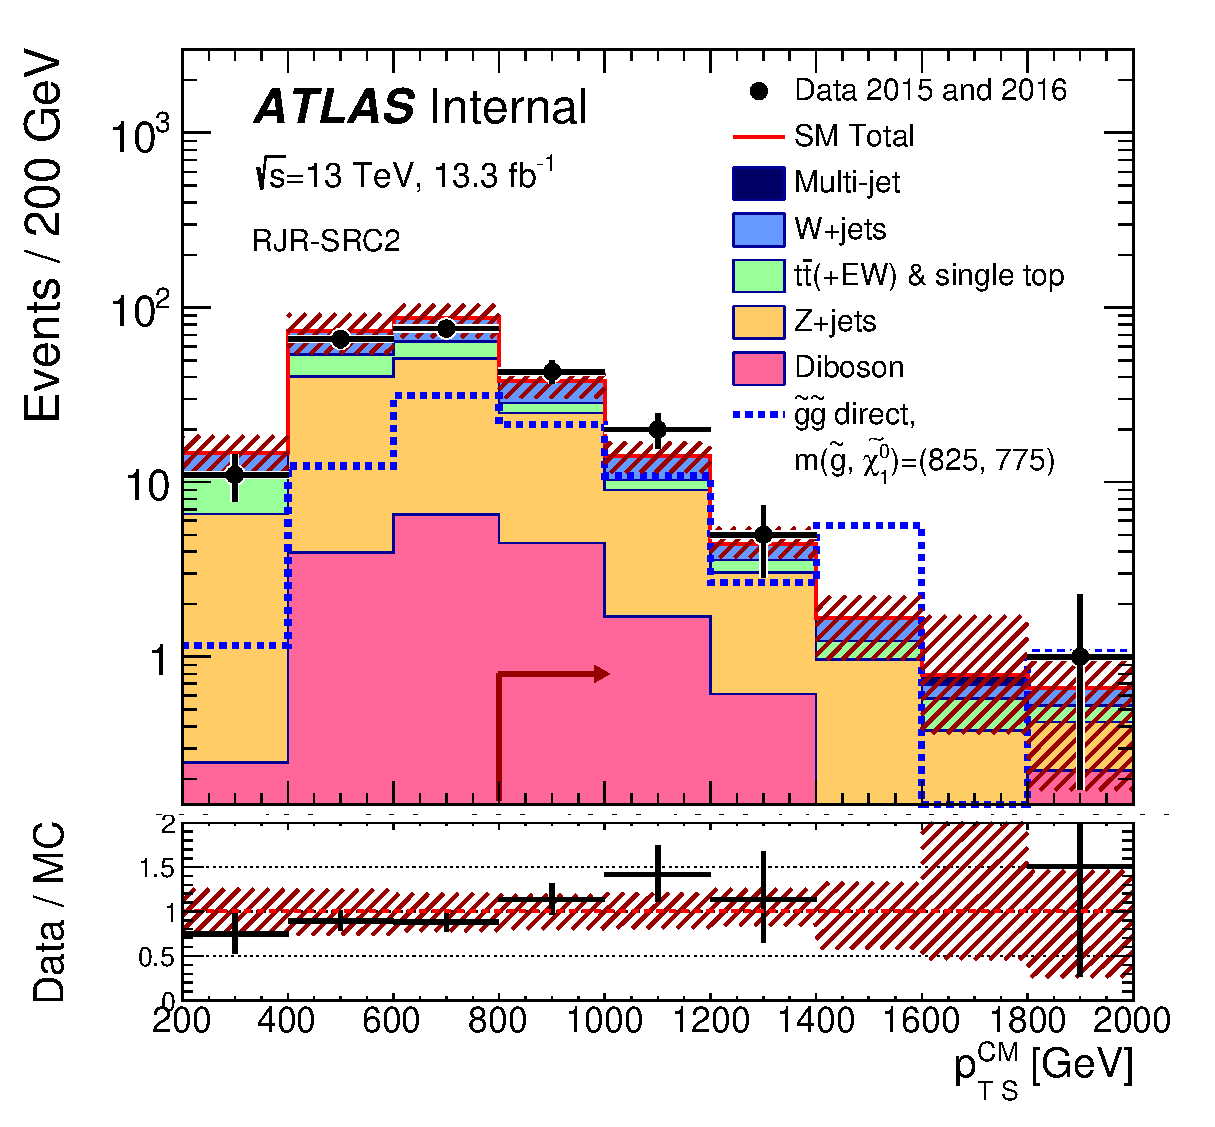
\includegraphics[width=0.45\textwidth]{ATLAS-CONF-2016-078_INT/N-1Plots/AtlasStyle/Preliminary/SR_SRJigsawSRC2_LastCut_SR_minusone}
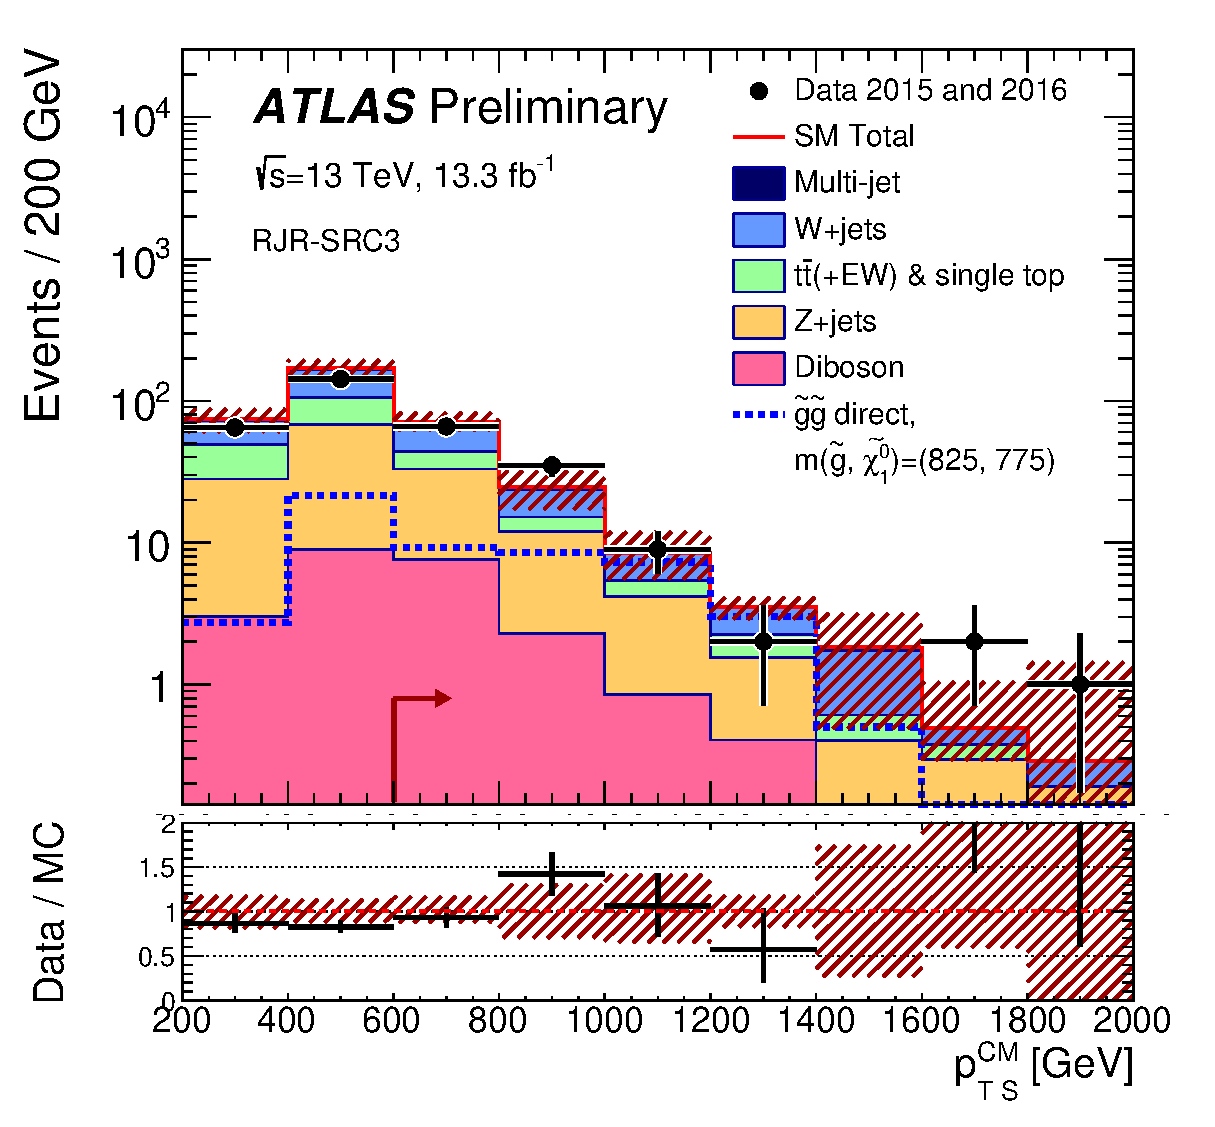
\includegraphics[width=0.45\textwidth]{ATLAS-CONF-2016-078_INT/N-1Plots/AtlasStyle/Preliminary/SR_SRJigsawSRC3_LastCut_SR_minusone}
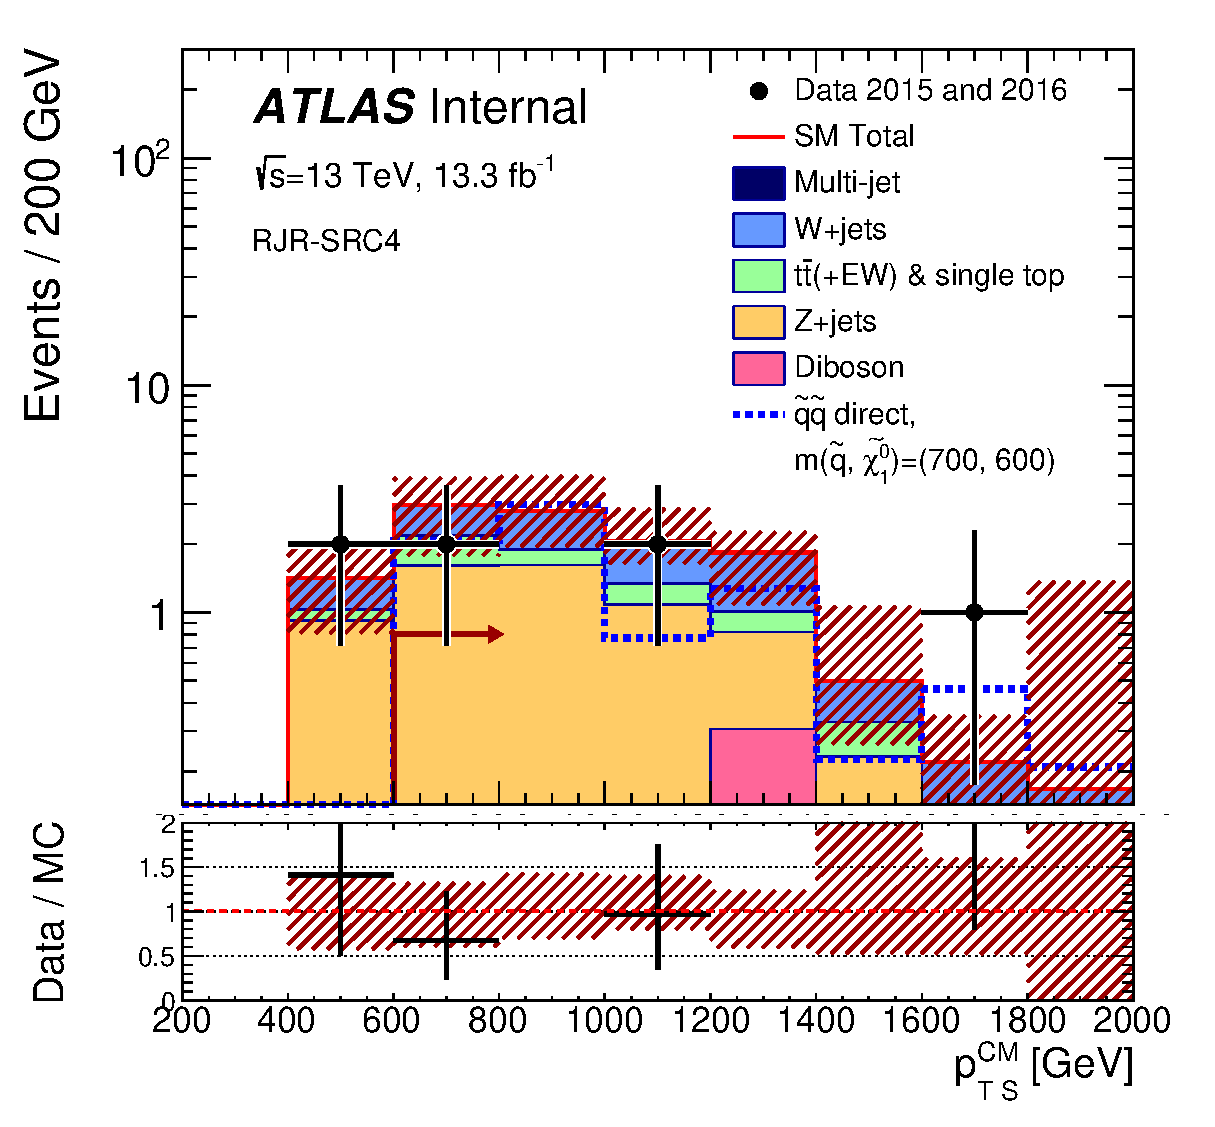
\includegraphics[width=0.45\textwidth]{ATLAS-CONF-2016-078_INT/N-1Plots/AtlasStyle/Preliminary/SR_SRJigsawSRC4_LastCut_SR_minusone}
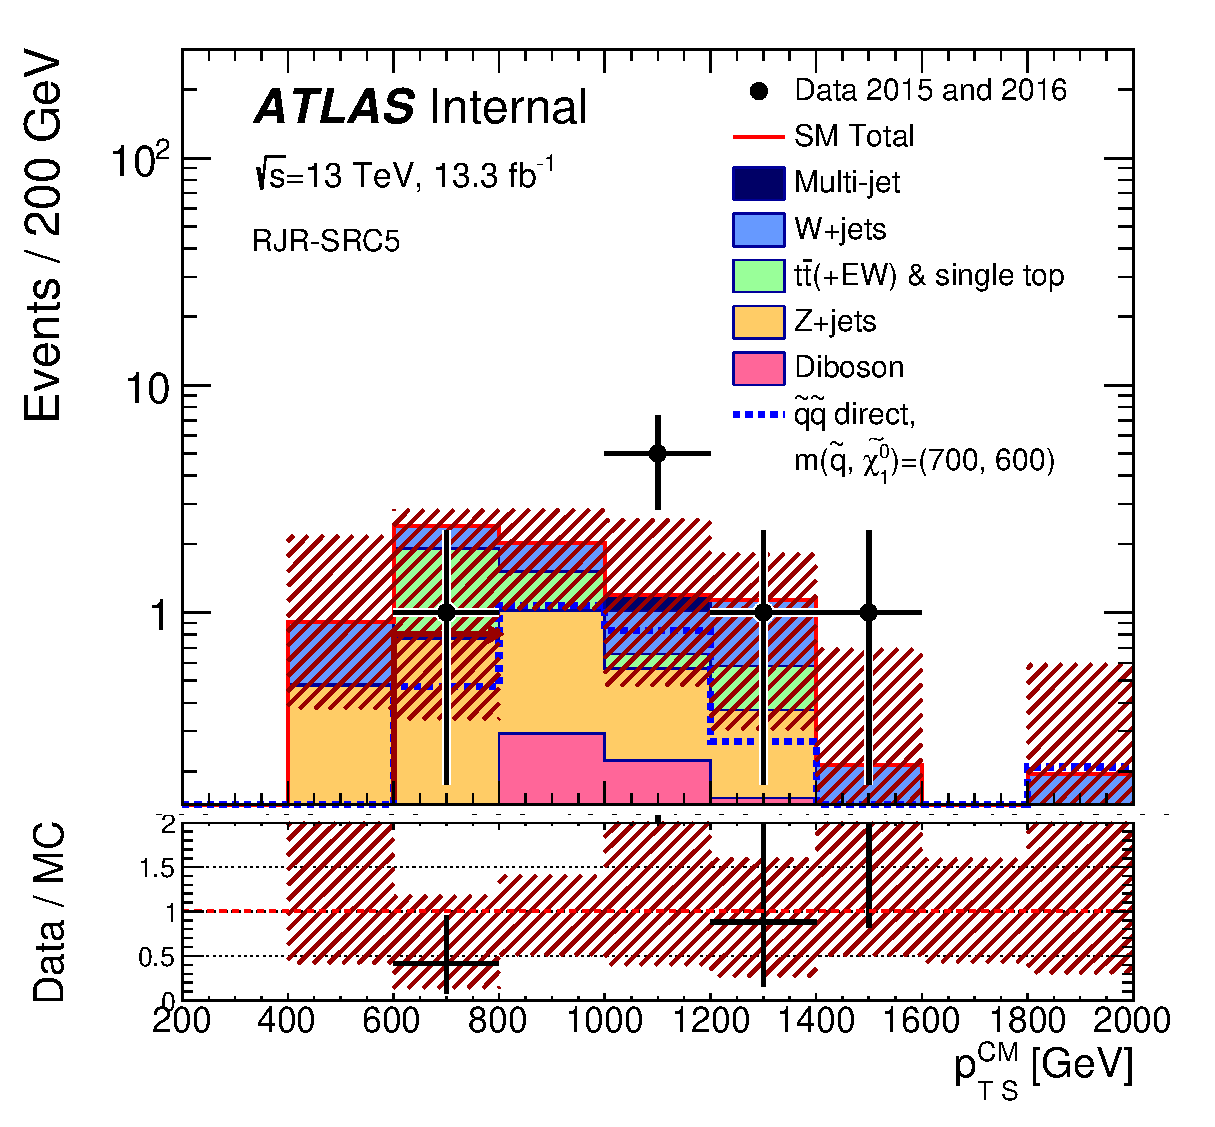
\includegraphics[width=0.45\textwidth]{ATLAS-CONF-2016-078_INT/N-1Plots/AtlasStyle/Preliminary/SR_SRJigsawSRC5_LastCut_SR_minusone}
\end{center}
\caption{}
\label{fig:src_scale}
\end{figure}

\begin{figure}[tbph]
\begin{center}
\includegraphics[width=0.45\textwidth]{ATLAS-CONF-2016-078_INT/N-1Plots/AtlasStyle/Preliminary/SR_SRJigsawSRG1a_LastCut_SR_minusone}
\includegraphics[width=0.45\textwidth]{ATLAS-CONF-2016-078_INT/N-1Plots/AtlasStyle/Preliminary/SR_SRJigsawSRG2a_LastCut_SR_minusone}
\includegraphics[width=0.45\textwidth]{ATLAS-CONF-2016-078_INT/N-1Plots/AtlasStyle/Preliminary/SR_SRJigsawSRG3a_LastCut_SR_minusone}
\end{center}
\caption{}
\label{fig:srg_scale}
\end{figure}

\begin{figure}[tbph]
\begin{center}
\includegraphics[width=0.45\textwidth]{ATLAS-CONF-2016-078_INT/N-1Plots/AtlasStyle/Preliminary/SR_SRJigsawSRS1a_LastCut_SR_minusone}
\includegraphics[width=0.45\textwidth]{ATLAS-CONF-2016-078_INT/N-1Plots/AtlasStyle/Preliminary/SR_SRJigsawSRS2a_LastCut_SR_minusone}
\includegraphics[width=0.45\textwidth]{ATLAS-CONF-2016-078_INT/N-1Plots/AtlasStyle/Preliminary/SR_SRJigsawSRS3a_LastCut_SR_minusone}
\end{center}
\caption{}
\label{fig:srs_scale}
\end{figure}


\section{Systematic uncertainties}

A table showing the full \ref{tab:BreakdownSysSRCompressed_RJR}.

%% This table is automatically generated from individual tables per signal region
%% you can update it via the script: ./makeAllSystTableInOne.py

\begin{table}[tbp]
%\small
\scriptsize
\begin{center}
%\begin{sidewaystable}
%\scriptsize
%\begin{center}
%\setlength{\tabcolsep}{0.0pc}
\begin{tabular}{|lrrrrrr|}
\hline
Channel  &  \textbf{ S1a } & \textbf{ S1b } & \textbf{ S2a } & \textbf{ S2b } & \textbf{ S3a } & \textbf{ S3b }  \\ \hline
Total bkg  &  $334$  &  $233$  &  $96$  &  $75$  &  $56$  &  $37$ \\
Total bkg unc.  &  $\pm 35$  [$10\%$]  &  $\pm 25$  [$11\%$]  &  $\pm 10$  [$10\%$]  &  $\pm 8$  [$11\%$]  &  $\pm 6$  [$11\%$]  &  $\pm 4$  [$11\%$] \\
\hline
MC statistics  &   --    &  $\pm 2.6$ [$1\%$]  &  $\pm 1.5$ [$2\%$]  &  $\pm 1.3$ [$2\%$]  &  $\pm 1.0$ [$2\%$]  &  $\pm 0.7$ [$2\%$] \\
$\Delta\mu_{Z,\mathrm{+jets}}$    &  $\pm 20$ [$6\%$]  &  $\pm 14$ [$6\%$]  &  $\pm 4$ [$4\%$]  &  $\pm 2.9$ [$4\%$]  &  $\pm 2.2$ [$4\%$]  &  $\pm 1.5$ [$4\%$] \\
$\Delta\mu_{W,\mathrm{+jets}}$    &  $\pm 10$ [$3\%$]  &  $\pm 7$ [$3\%$]  &  $\pm 3.1$ [$3\%$]  &  $\pm 2.3$ [$3\%$]  &  $\pm 1.6$ [$3\%$]  &  $\pm 1.1$ [$3\%$] \\
$\Delta\mu_{  \mathrm{ Top}}$       &  $\pm 6$ [$2\%$]  &  $\pm 4$ [$2\%$]  &  $\pm 1.5$ [$2\%$]  &  $\pm 1.1$ [$1\%$]  &  $\pm 0.9$ [$2\%$]  &  $\pm 0.6$ [$2\%$] \\
$\Delta\mu_{  \mathrm{ Multijet}}$  &  $\pm 0.09$ [$0\%$]  &  $\pm 0.05$ [$0\%$]  &  $\pm 0.02$ [$0\%$]  &   --    &   --    &   --   \\
CR$\gamma$ corr. factor  &  $\pm 12$ [$4\%$]  &  $\pm 8$ [$3\%$]  &  $\pm 4$ [$4\%$]  &  $\pm 2.9$ [$4\%$]  &  $\pm 2.2$ [$4\%$]  &  $\pm 1.4$ [$4\%$] \\
Theory Z  &  $\pm 23$ [$7\%$]  &  $\pm 16$ [$7\%$]  &  $\pm 7$ [$7\%$]  &  $\pm 6$ [$8\%$]  &  $\pm 4$ [$7\%$]  &  $\pm 2.8$ [$8\%$] \\
Theory W  &  $\pm 4$ [$1\%$]  &  $\pm 5$ [$2\%$]  &  $\pm 0.4$ [$0\%$]  &  $\pm 0.11$ [$0\%$]  &  $\pm 1.5$ [$3\%$]  &  $\pm 1.2$ [$3\%$] \\
Theory Top   &  $\pm 4$ [$1\%$]  &  $\pm 2.7$ [$1\%$]  &  $\pm 0.8$ [$1\%$]  &  $\pm 0.7$ [$1\%$]  &  $\pm 0.6$ [$1\%$]  &  $\pm 0.4$ [$1\%$] \\
Theory Diboson  &  $\pm 9$ [$3\%$]  &  $\pm 6$ [$3\%$]  &  $\pm 2.8$ [$3\%$]  &  $\pm 2.6$ [$3\%$]  &  $\pm 2.1$ [$4\%$]  &  $\pm 1.4$ [$4\%$] \\
Jet/MET   &  $\pm 3.3$ [$1\%$]  &  $\pm 1.5$ [$1\%$]  &  $\pm 0.6$ [$1\%$]  &  $\pm 0.6$ [$1\%$]  &  $\pm 1.2$ [$2\%$]  &  $\pm 1.0$ [$3\%$] \\
Multijet method  &  $\pm 0.7$ [$0\%$]  &  $\pm 0.4$ [$0\%$]  &  $\pm 0.08$ [$0\%$]  &   --    &   --    &   --   \\
\hline
\end{tabular}

\begin{tabular}{|lrrrrrr|}
\hline
Channel  &  \textbf{ G1a } & \textbf{ G1b } & \textbf{ G2a } & \textbf{ G2b } & \textbf{ G3a } & \textbf{ G3b }  \\ \hline
Total bkg  &  $40$  &  $18.8$  &  $27.8$  &  $8.5$  &  $5.8$  &  $1.7$ \\
Total bkg unc.  &  $\pm 4$  [$10\%$]  &  $\pm 2.5$  [$13\%$]  &  $\pm 3.4$  [$12\%$]  &  $\pm 1.4$  [$16\%$]  &  $\pm 1.1$  [$19\%$]  &  $\pm 0.4$  [$24\%$] \\
\hline
MC statistics  &  $\pm 1.6$ [$4\%$]  &  $\pm 1.0$ [$5\%$]  &  $\pm 1.2$ [$4\%$]  &  $\pm 0.6$ [$7\%$]  &  $\pm 0.4$ [$7\%$]  &  $\pm 0.23$ [$14\%$] \\
$\Delta\mu_{Z,\mathrm{+jets}}$  &  $\pm 1.5$ [$4\%$]  &  $\pm 0.7$ [$4\%$]  &  $\pm 1.6$ [$6\%$]  &  $\pm 0.5$ [$6\%$]  &  $\pm 0.4$ [$7\%$]  &  $\pm 0.1$ [$6\%$] \\
$\Delta\mu_{W,\mathrm{+jets}}$  &  $\pm 0.9$ [$2\%$]  &  $\pm 0.4$ [$2\%$]  &  $\pm 1.2$ [$4\%$]  &  $\pm 0.31$ [$4\%$]  &  $\pm 0.28$ [$5\%$]  &  $\pm 0.1$ [$6\%$] \\
$\Delta\mu_{\mathrm{ Top}}$  &  $\pm 0.8$ [$2\%$]  &  $\pm 0.33$ [$2\%$]  &  $\pm 0.9$ [$3\%$]  &  $\pm 0.23$ [$3\%$]  &  $\pm 0.07$ [$1\%$]  &  $\pm 0.1$ [$6\%$] \\
$\Delta\mu_{\mathrm{ Multijet}}$  &  $\pm 0.1$ [$0\%$]  &  --  &  $\pm 0.03$ [$0\%$]  &  $\pm 0.02$ [$0\%$]  &   --    &   --   \\
CR$\gamma$ corr. factor  &  $\pm 1.2$ [$3\%$]  &  $\pm 0.6$ [$3\%$]  &  $\pm 0.8$ [$3\%$]  &  $\pm 0.26$ [$3\%$]  &  $\pm 0.19$ [$3\%$]  &  $\pm 0.05$ [$3\%$] \\
Theory Z  &  $\pm 2.3$ [$6\%$]  &  $\pm 1.1$ [$6\%$]  &  $\pm 1.6$ [$6\%$]  &  $\pm 0.5$ [$6\%$]  &  $\pm 0.4$ [$7\%$]  &  $\pm 0.1$ [$6\%$] \\
Theory W  &  $\pm 1.1$ [$3\%$]  &  $\pm 1.3$ [$7\%$]  &  $\pm 0.3$ [$1\%$]  &  $\pm 0.7$ [$8\%$]  &  $\pm 0.6$ [$10\%$]  &  $\pm 0.16$ [$9\%$] \\
Theory Top   &  $\pm 1.2$ [$3\%$]  &  $\pm 0.7$ [$4\%$]  &  $\pm 1.0$ [$4\%$]  &  $\pm 0.4$ [$5\%$]  &  $\pm 0.4$ [$7\%$]  &  $\pm 0.26$ [$15\%$] \\
Theory Diboson  &  $\pm 1.3$ [$3\%$]  &  $\pm 0.8$ [$4\%$]  &  $\pm 1.5$ [$5\%$]  &  $\pm 0.6$ [$7\%$]  &  $\pm 0.31$ [$5\%$]  &  $\pm 0.13$ [$8\%$] \\
Jet/MET   &  $\pm 1.0$ [$3\%$]  &  $\pm 0.6$ [$3\%$]  &  $\pm 0.4$ [$1\%$]  &  $\pm 0.17$ [$2\%$]  &  $\pm 0.22$ [$4\%$]  &  $\pm 0.05$ [$3\%$] \\
Multijet method  &  $\pm 0.24$ [$1\%$]  &  $\pm 0.12$ [$1\%$]  &  $\pm 0.5$ [$2\%$]  &  $\pm 0.4$ [$5\%$]  &   --    &   --   \\
\hline
\end{tabular}

\begin{tabular}{|lrrrrr|}
\hline
Channel                           & \textbf{ C1 }   & \textbf{ C2 }  & \textbf{ C3 }  & \textbf{ C4 }   & \textbf{ C5 }   \\ \hline
Total bkg                         & $14.5$              & $59$               & $110$              & $10.5$              & $7.3$               \\
Total bkg unc.                    & $\pm 2.2$  [$15\%$] & $\pm 6$  [$10\%$]  & $\pm 11$  [$10\%$] & $\pm 1.5$  [$14\%$] & $\pm 1.4$  [$19\%$] \\
\hline
MC statistics                     & $\pm 0.7$ [$5\%$]   & $\pm 1.7$ [$3\%$]  & $\pm 2.4$ [$2\%$]  & $\pm 0.6$ [$6\%$]   & $\pm 0.6$ [$8\%$]   \\
$\Delta\mu_{Z,\mathrm{+jets}}$    & $\pm 0.5$ [$3\%$]   & $\pm 1.9$ [$3\%$]  & $\pm 2.5$ [$2\%$]  & $\pm 0.31$ [$3\%$]  & $\pm 0.13$ [$2\%$]  \\
$\Delta\mu_{W,\mathrm{+jets}}$    & $\pm 0.4$ [$3\%$]   & $\pm 1.7$ [$3\%$]  & $\pm 5$ [$5\%$]    & $\pm 0.4$ [$4\%$]   & $\pm 0.25$ [$3\%$]  \\
$\Delta\mu_{\mathrm{ Top}}$       & $\pm 0.33$ [$2\%$]  & $\pm 1.3$ [$2\%$]  & $\pm 4$ [$4\%$]    & $\pm 0.31$ [$3\%$]  & $\pm 0.4$ [$5\%$]   \\
$\Delta\mu_{\mathrm{ Multijet}}m$ & --                  & $\pm 0.1$ [$0\%$]  & $\pm 0.06$ [$0\%$] & --                  & $\pm 0.1$ [$1\%$]   \\
CR$\gamma$ corr. factor $\kappa$  & $\pm 0.5$ [$3\%$]   & $\pm 1.8$ [$3\%$]  & $\pm 2.3$ [$2\%$]  & $\pm 0.29$ [$3\%$]  & $\pm 0.13$ [$2\%$]  \\
Theory Z                          & $\pm 0.8$ [$6\%$]   & $\pm 3.5$ [$6\%$]  & $\pm 4$ [$4\%$]    & $\pm 0.6$ [$6\%$]   & $\pm 0.24$ [$3\%$]  \\
Theory W                          & $\pm 1.3$ [$9\%$]   & $\pm 0.03$ [$0\%$] & $\pm 2.0$ [$2\%$]  & $\pm 1.0$ [$10\%$]  & $\pm 0.13$ [$2\%$]  \\
Theory Top                        & $\pm 0.5$ [$3\%$]   & $\pm 1.3$ [$2\%$]  & $\pm 3.2$ [$3\%$]  & $\pm 0.6$ [$6\%$]   & $\pm 0.9$ [$12\%$]  \\
Theory Diboson                    & $\pm 1.0$ [$7\%$]   & $\pm 4$ [$7\%$]    & $\pm 6$ [$5\%$]    & $\pm 0.27$ [$3\%$]  & $\pm 0.4$ [$5\%$]   \\
Jet/MET                           & $\pm 0.5$ [$3\%$]   & $\pm 1.5$ [$3\%$]  & $\pm 3.1$ [$3\%$]  & $\pm 0.24$ [$2\%$]  & $\pm 0.5$ [$7\%$]   \\
Multijet method                   & $\pm 0.09$ [$1\%$]  & $\pm 0.4$ [$1\%$]  & $\pm 2.1$ [$2\%$]  & --                  & $\pm 0.18$ [$2\%$]  \\
\hline
\end{tabular}

%\end{tabular*}
\end{center}
\caption{
Breakdown of the dominant systematic uncertainties in the background estimates.
The individual uncertainties can be correlated, and do not necessarily add in quadrature.
$\Delta_{\mu}$ uncertainties result from control region statistical uncertainties and the systematic uncertainties in the appropriate control region.
In brackets, uncertainties are given relative to the expected total background yield, also presented in the Table. Empty cells (indicated by a `-') correspond to uncertainties $<$0.1\%. \label{tab:BreakdownSysSRCompressed_RJR}}
%\end{sidewaystable}
\end{table}


\section{Pull Plots}

\section{Exclusion plots}
